\documentclass[tikz,border=4pt]{standalone}
\usepackage{amsmath}
\begin{document}
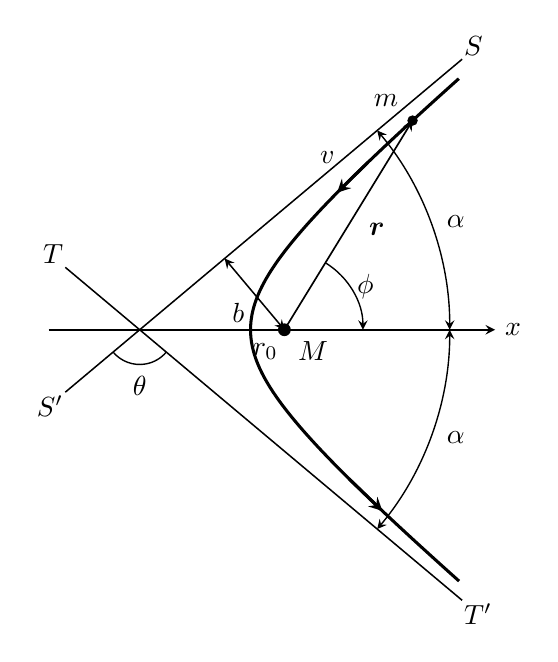
\begin{tikzpicture}[>=stealth, thick, scale=1.05]
  % Exact hyperbola parameters: alpha = 40 deg => e = 1/cos(40) = 1.30541
  % Center at (-c, 0) with c = 1.75 => a = c/e = 1.34058, b = c*sin(40) = 1.12488
  % Vertex (periapsis) at (-c + a, 0) = (-0.40942, 0), Focus M at (0, 0)
  % Asymptotes: y = +/- tan(40)*(x + 1.75) = +/- 0.83910*(x + 1.75)
  \def\ch{1.75}
  \def\ah{1.34058}
  \def\bh{1.12488}
  \def\tana{0.83910}

  % x-axis
  \draw[->, line width=0.55pt] (-2.85, 0) -- (2.55, 0) node[right] {$x$};

  % Asymptotes SS' and TT'
  \draw[line width=0.55pt] (-2.65, {\tana*(-2.65 + \ch)}) -- (2.15, {\tana*(2.15 + \ch)});
  \draw[line width=0.55pt] (-2.65, {-\tana*(-2.65 + \ch)}) -- (2.15, {-\tana*(2.15 + \ch)});
  \node[below left] at (-2.55, {\tana*(-2.55 + \ch)}) {$S'$};
  \node[above right] at (2.05, {\tana*(2.05 + \ch)}) {$S$};
  \node[above left] at (-2.55, {-\tana*(-2.55 + \ch)}) {$T$};
  \node[below right] at (2.05, {-\tana*(2.05 + \ch)}) {$T'$};

  % Hyperbolic trajectory: x(s) = -c + a*cosh(s), y(s) = b*sinh(s)
  \draw[line width=1.1pt, domain=-1.72:1.72, samples=120]
    plot ({-\ch + \ah*cosh(\x)}, {\bh*sinh(\x)});

  % Direction arrows along incoming and outgoing branches
  \draw[->, line width=1.1pt]
    ({-\ch + \ah*cosh(1.35)}, {\bh*sinh(1.35)}) -- ({-\ch + \ah*cosh(1.18)}, {\bh*sinh(1.18)});
  \draw[->, line width=1.1pt]
    ({-\ch + \ah*cosh(-1.25)}, {\bh*sinh(-1.25)}) -- ({-\ch + \ah*cosh(-1.42)}, {\bh*sinh(-1.42)});

  % Planet M at origin
  \fill (0, 0) circle (2.2pt);
  \node[below right] at (0.04, -0.02) {$M$};

  % Probe m on incoming branch at s = 1.55
  % x(1.55) = -1.75 + 1.34058*2.46186 = 1.5503, y(1.55) = 1.12488*2.24961 = 2.5305
  \pgfmathsetmacro{\mx}{-\ch + \ah*cosh(1.55)}
  \pgfmathsetmacro{\my}{\bh*sinh(1.55)}
  \fill (\mx, \my) circle (1.8pt);
  \node[above left] at (\mx - 0.05, \my + 0.05) {$m$};
  \node[above left] at ({-\ch + \ah*cosh(1.25) - 0.05}, {\bh*sinh(1.25) + 0.08}) {$v$};

  % Position vector r from M to m
  \draw[->, line width=0.6pt] (0, 0) -- (\mx, \my);
  \node[below right] at (0.58*\mx, 0.56*\my) {$\boldsymbol{r}$};

  % Angle phi from +x axis to r (atan2(my, mx) = 58.5 deg)
  \draw[<-, line width=0.5pt] (0.95, 0) arc[start angle=0, end angle=58.5, radius=0.95];
  \node at (0.98, 0.52) {$\phi$};

  % Impact parameter b: perpendicular from M(0,0) to SS'
  % Foot: (-c*sin^2(40), c*sin(40)*cos(40)) = (-0.72306, 0.86171)
  \draw[<->, line width=0.55pt] (0, 0) -- (-0.723, 0.862);
  \node[below left] at (-0.36, 0.44) {$b$};

  % Closest approach r0 from periapsis (-0.409, 0) to M(0,0)
  \node[below] at (-0.23, -0.04) {$r_0$};

  % Angle theta between S' and T' at intersection (-1.75, 0)
  % S' direction is 220 deg, T' direction is 320 deg
  \draw[line width=0.5pt] (-\ch, 0) ++(220:0.42) arc[start angle=220, end angle=320, radius=0.42];
  \node[below] at (-\ch, -0.44) {$\theta$};

  % Angles alpha between +x axis and asymptotes
  \draw[<->, line width=0.5pt] (-\ch, 0) ++(0:3.75) arc[start angle=0, end angle=40, radius=3.75];
  \node[right] at ({-\ch + 3.82*cos(20)}, {3.82*sin(20)}) {$\alpha$};
  \draw[<->, line width=0.5pt] (-\ch, 0) ++(0:3.75) arc[start angle=0, end angle=-40, radius=3.75];
  \node[right] at ({-\ch + 3.82*cos(-20)}, {3.82*sin(-20)}) {$\alpha$};
\end{tikzpicture}
\end{document}
